\documentclass[twocolumn]{article}

\usepackage[utf8]{inputenc}
\usepackage[T1]{fontenc}
\usepackage{amsmath}
\usepackage{amsthm}
\usepackage{graphicx}
\usepackage{breqn}

\newtheorem{lemma}{Lemma}
\newtheorem{theorem}{Theorem}

\newcommand{\beq}{\begin{eqnarray}}
\newcommand{\eeq}{\end{eqnarray}}

\title{DRAFT: Robust Communication in Structured Networks}
\author{
    Edward L. Platt\\
    elplatt@umich.edu
    \and
    Daniel M. Romero\\
    drom@umich.edu
}
\date{December 2015}

\begin{document}

\maketitle

\section{Introduction}

\section{Trust Model}

We assume that a sender $A$ (or Alice) wants to send sensitive information
to a receiver $B$ (or Bob).
Alice and Bob are both nodes on a communication network represented by a graph
$G = (V, E)$.
Two nodes are connected when they are able to communicate directly with each
other.
We also assume the presence of an adversary $C$ (or Eve) who wishes to disrupt
that communication by altering or delaying the transmission.
Eve has compromised a subset of nodes and has full control over their behavior.
Any transmission routed through a compromised node is considered faulty.
Alice and Bob do not know which nodes have been compromised.

In our model, links also represent trust.
Specifically, two nodes are connected if each node believes that the other
has not been compromised by its adversary.
In other words, a communication link is severed if one node believes the other
to be compromised.
If trust were transitive, a connected path from Alice to Bob, would guarantee
a trusted channel, but trust is not transitive \cite{christianson_why_1997}.
Rather than entirely abandoning transisitivy, we assume that trust is
partially transitive.
Specifically each node has a {\em trusted neighborhood} of nodes up to $h$ hops
away, which we assume have not been compromised by that node's adversaries.
Our objective is now to construct a robust communication channel from Alice's
trusted neighborhood to Bob's.

\section{Multipath Fault Tolerance}

We achieve robust communication between trusted neighborhoods through
Concurrent Multipath Routing (CMR) \cite{}.
If there are multiple {\em redundant paths} (i.e., paths sharing no nodes or
links) between Alice and Bob's trusted neighborhoods, multiple copies of a
message can be sent along different paths, enabling standard error detection and
error correction techniques to be applied at the destination.
If Alice randomly selects $k$ of $n$ total redundant paths, Eve's best strategy
is to compromise at least one node on as many of the paths as possible.
Because an error can be detected if even a single copy has been tampered with,
Eve must compromise all $k$ paths in order to convince Bob to accept a compromised
message.
If Eve has the resources to compromise $l$ total nodes, the probability that
Bob receives an undetectable error is:
\beq
\label{eq:pe}
p_e &=& \frac{l!(n-k)!}{n!(l-k)!}.
\eeq
Letting $k=\alpha n$ and $l=\beta n$, then applying Stirling's
approximation gives:
\begin{eqnarray}
\nonumber
p_e &\approx&
\frac{\sqrt{\beta(1-\alpha)}}{\sqrt{\beta-\alpha}} \\
& &
\times {}
\label{eq:pe_approx}
\left[
    \left( \frac{\beta-\alpha}{1-\alpha} \right)^{\alpha}
    \left( \frac{\beta}{\beta-\alpha} \right)^{\beta}
    (1-\alpha)
\right]^n
\end{eqnarray}
Note that Eq. (\ref{eq:pe_approx}) is exponential in the number of redundant
paths $n$, which depends only on the network structure, and not on the
resources available to individual nodes.
If a network has a large number of redundant paths between trusted neighborhoods,
a very low probability of undetected errors can be achieved, even if an adversary
has the resources to compromise a very large fraction of the avialable paths.
The value of $p_e$ for various $k$, $l$, and $n$ is shown in Figure
\ref{fig:perror}.

\begin{figure}
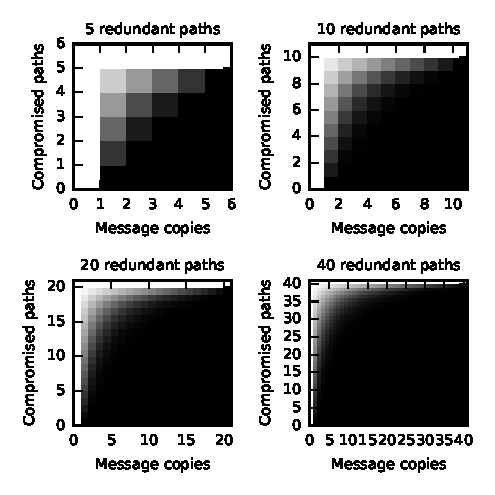
\includegraphics{fig-perror.pdf}
\caption{
Probability $p_e$ of an undetected error as a function of the number of message
copies $k$ and compromised paths $l$.
\label{fig:perror}
}
\end{figure}

\section{Butterfly Network}

\begin{figure}
\begin{center}
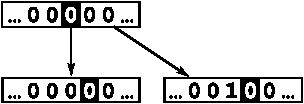
\includegraphics{fig-butterfly.pdf}
\end{center}
\caption{
\label{fig:butterfly}
}
\end{figure}

\section{Discussion}

\section{Conclusion}

\bibliographystyle{plain}
\bibliography{netft}

\end{document}
